\documentclass[12pt, twoside]{article}
\usepackage[letterpaper, margin=1in, headsep=0.5in]{geometry}
\usepackage[english]{babel}
\usepackage[utf8]{inputenc}
\usepackage{amsmath}
\usepackage{amsfonts}
\usepackage{amssymb}
\usepackage{tikz}
\usepackage{yhmath}
%\usetikzlibrary{quotes, angles}

\usepackage{graphicx}
\usepackage{enumitem}
\usepackage{multicol}

\usepackage{fancyhdr}
\pagestyle{fancy}
\fancyhf{}
\renewcommand{\headrulewidth}{0pt} % disable the underline of the header

\fancyhead[RE]{\thepage}
\fancyhead[RO]{\thepage \\ Name: \hspace{3cm}}
\fancyhead[L]{BECA / Dr. Huson / 10th Grade Geometry\\* 12 June 2019}

\begin{document}
\subsubsection*{13.9 Do Now: Circle situations \& trigonometry}
Use only a compass and straightedge for these constructions. [show all compass marks]
  \begin{enumerate}

  \item Bisect the given angle. \vspace{1cm}
    \begin{center}
    \begin{tikzpicture}
      \draw [<->, thick] (20:6)--(0,0)--(-100:5);
      \draw [fill] (0,0) circle [radius=0.05] node[left]{$A$};
    \end{tikzpicture}
  \end{center} \vspace{0.5cm}

  \item Construct a median to $\overline{AB}$ from $C$.\\
    \vspace{3cm}
    \begin{center}
    \begin{tikzpicture}
      \draw [<->, thick] (0,0)--(10,0)--(6,-3)--cycle;
      \draw [fill] (0,0) circle [radius=0.05] node[left]{$A$};
      \draw [fill] (10,0) circle [radius=0.05] node[right]{$B$};
      \draw [fill] (6,-3) circle [radius=0.05] node[below right]{$C$};
    \end{tikzpicture}
  \end{center}

\newpage
Show the calculation. When rounding, write down the full calculator display first.
   \item What is the area of a circle with diameter 22, rounded to the \emph{nearest tenth}? \vspace{2.5cm}
   \item What is the circumference of a circle with radius 7, rounded to the \emph{nearest tenth}? \vspace{2.5cm}
   \item What is the radius of a circle with circumference 100.5, rounded to the \emph{nearest hundredth}? \vspace{4cm}

  \item Circle $O$ has a radius $AO=11$ cm, as shown below, and arc measure $m \wideparen{AB}=105^\circ$.
     \begin{multicols}{2}
       \begin{tikzpicture}[scale=.6]
         \draw (0,0) circle[radius=5];
         \draw [thick]
         (-30:5) node[right] {$A$}--(0,0);
         \draw [thick] (0,0)--(90:5) node[above] {$B$};
         \fill (0,0) circle[radius=0.1] node[below]{$O$};
         \draw (15:6) node{$105^\circ$};
         \draw (-35:2.5) node[below]{$11$};
         %\draw (75:1.8) node[above] {$C$};
         %\draw (290:5) node[below] {$D$};
       \end{tikzpicture}
     \columnbreak
       \begin{enumerate}
         \item Find the $m \angle AOB$. \vspace{1cm}
         \item Find the length of the arc $\wideparen{AB}$ to the \emph{nearest tenth}. \vspace{3cm}
         \item Find the area of the sector $AOB$ to the \emph{nearest tenth}. %\vspace{2.5cm}
       \end{enumerate}
     \end{multicols}


\newpage
\raggedcolumns
  \item Right $\triangle ABC$ has sides of length $BC=8$, $AC=15$, and $AB=17$ as shown. %\vspace{0.5cm}
  \begin{multicols}{2}
            Find to the \emph{nearest thousandth}.
        \begin{enumerate}
          \item $\sin A =$ \vspace{1cm}
          \item $\tan A =$ \vspace{1cm}
          \item $\tan B =$ \vspace{1cm}
          \item Find $m\angle A$ to the \emph{nearest degree}. \vspace{1cm}
      \end{enumerate}
      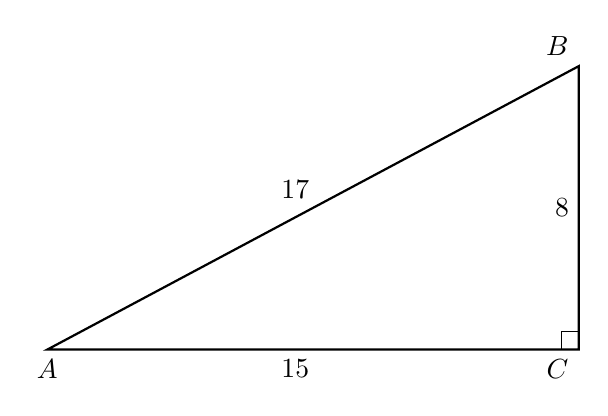
\begin{tikzpicture}[scale=0.45]
        \draw [thick]
        (0,0)node[below]{$A$}--
        (15,0)node[below left]{$C$}--
        (15,8)node[above left]{$B$}--cycle;
        \draw (15,0)++(-0.5,0)--++(0,0.5)--+(0.5,0);
        \node at (7,0)[below]{$15$};
        \node at (15,4)[left]{$8$};
        \node at (7,4)[above]{$17$};
      \end{tikzpicture}
    \end{multicols} \vspace{1cm}

  \item In a right triangle, the acute angles have the relationship $\sin (30)=\cos(x)$.\\[0.25cm]
    What is the value of $x$? \vspace{3cm}

  \item If $\sin (x-15)^\circ = \cos(55)^\circ$, what is the value of $x$? \vspace{5cm}

  \item Express each value to \emph{the nearest tenth}.  \vspace{0.5cm}
    \begin{multicols}{2}
      \begin{enumerate}
        \item $\tan 45^\circ = $ \vspace{1cm}
        \item $\cos 60^\circ =$
        \item $\tan^{-1} 1 = $ \vspace{1cm}
        \item $\sin^{-1} 0.866 =$
      \end{enumerate}
    \end{multicols}

\newpage

  \item A flag pole is 80 feet away, and the angle of elevation to its top is $32^\circ$. To the \emph{nearest foot}, what is the height of the pole?\\
   \begin{tikzpicture}[scale=1.1]
     \draw [dashed] (10,0)--(0,0)--(10,4);
     \draw [thick, ->] (10,0)--(10,4);
     \draw (10,0)++(-0.3,0)--++(0,0.3)--+(0.3,0);
     \fill [lightgray] (0,0)--(0.75,0) arc [start angle=0, end angle=22, radius=0.75]--cycle;
     \node at (1,0)[below]{$32^\circ$};
     \node at (10,2)[right]{Flag Pole};
     \node at (5,0)[below]{80 feet};
   \end{tikzpicture} \vspace{4cm}

   \item Right $\triangle ABC$ is drawn with point $D$ on $\overline{AC}$. $m\angle BAC=53^\circ$, $m\angle BDC=78^\circ$, $m\angle C=90^\circ$, and $AC=50$. \\[0.5cm]
   ``Solve the triangle": Find $BC$, $BD$, $CD$, and $AD$. \vspace{0.5cm}
       \begin{flushright}
         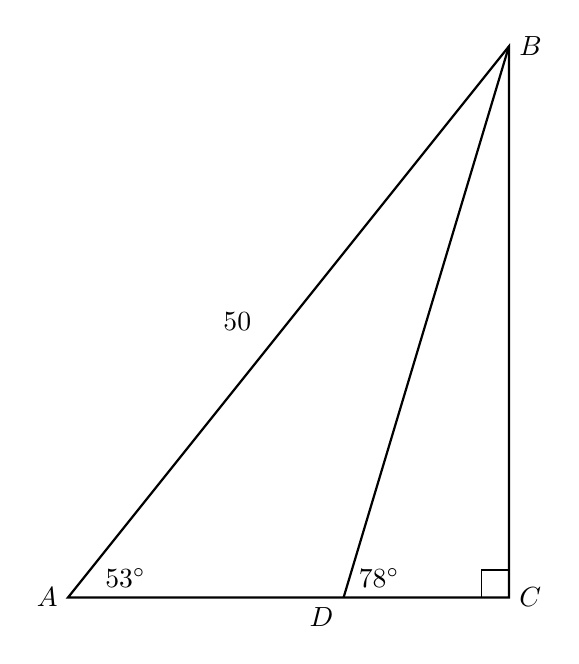
\begin{tikzpicture}[scale=0.7]
           \draw [thick] (-8,0)node[left]{$A$}
           --(0,0)node[right]{$C$}
           --(0,10)node[right]{$B$}--cycle;
           %\draw (0,0) circle [radius=5] node[below]{$O$};
           \draw [thick] (-3,0)node[below left]{$D$}--(0,10);
           \draw (0,0) ++(-180:0.5)-- ++(90:0.5)-- +(0:0.5);
           \node at (-4.5,5)[left]{$50$};
           \node at (-7.5,0)[above right]{$53^\circ$};
           \node at (-2.9,0)[above right]{$78^\circ$};
         \end{tikzpicture}
      \end{flushright}%\vspace{5cm}

\newpage
  \item Given circle $O$ with points $P$ and $Q$ on the circle. $m\angle POQ=110$. Find $m\angle P$.\\[1cm]
      %\hspace{1cm} Given the line  $l$ and point $P$.
      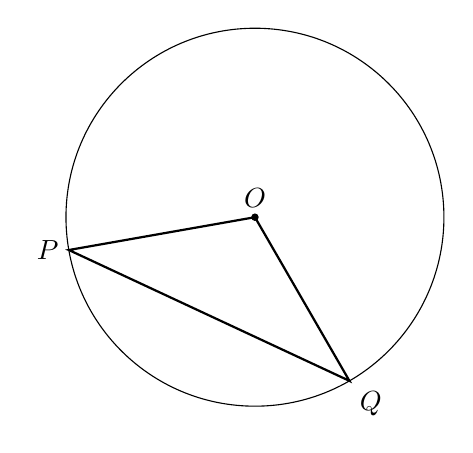
\begin{tikzpicture}[scale=0.8]
        %\draw [-, thick] (-6,0) node[left]{$A$}--(0,0);
        \draw  (0,0) circle [radius=3] node[above]{$O$};
        \draw [-, thick] (190:3) node[left]{$P$}--(0,0)
          --(300:3) node[below right]{$Q$}--cycle;
        %\node at (8.5,-0.4){$l$};
        \draw [fill] (0,0) circle [radius=0.05];
      \end{tikzpicture} %\vspace{3cm}

    \item A pyramid with a square base is 8 cm tall, as shown. The slant length, $VM=10$. Find the volume of the pyramid.\\[1cm]
    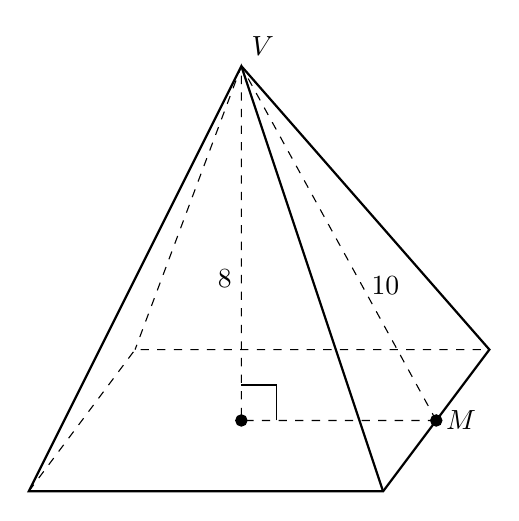
\begin{tikzpicture}[scale=0.9]
      \draw [thick] (-3,-1)--(2,-1)--(3.5,1)--(0,5)node[above right]{$V$}
        --cycle;
      \draw [dashed] (-3,-1)--(-1.5,1)--(3.5,1);
      \draw [thick] (2,-1)--(0,5);
      \draw [dashed] (2.75,0)
        --(0,0)--(0,5)--(-1.5,1);
      \draw (0,0) ++(0:0.5)-- ++(90:0.5)-- +(180:0.5);
      \draw [dashed] (2.75,0)--(0,5);
      \draw [fill] (0,0) circle [radius=0.08];
      \draw [fill] (2.75,0) circle [radius=0.08]node[right]{$M$};
      \node at (0,2)[left]{8};
      \node at (1.7,1.9)[right]{10};
    \end{tikzpicture}

\newpage
  \item Circle $O$ has a tangent lines $\overleftrightarrow{PT}$ with point of tangency $T$ and $\overleftrightarrow{PS}$ with point of tangency $S$, as shown. If $OP=13$ and the radius of circle $O$ is $5$, what is the perimeter of quadrilateral $PSOT$? \vspace{0.5cm}
    \begin{center}
      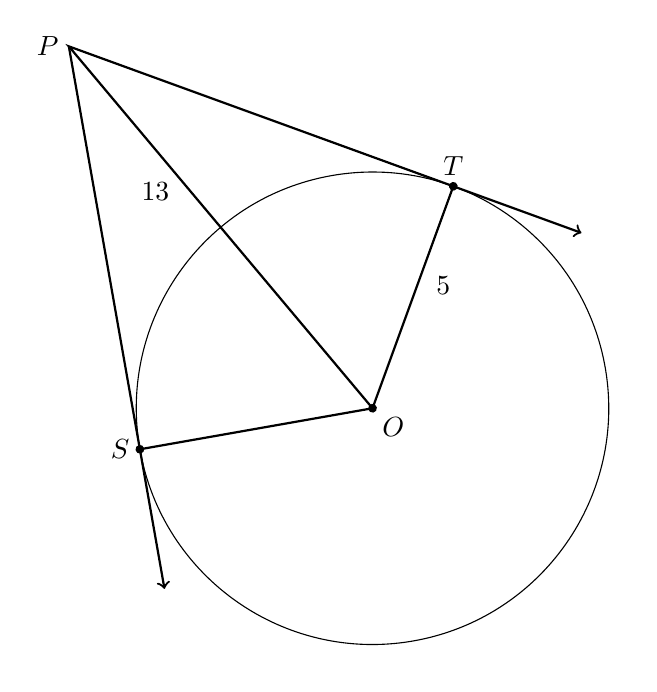
\begin{tikzpicture}[scale=0.6, rotate=-80]
        \draw [<-, thick] (120:5.774)--(210:10)node[left]{$P$}
        --(0,0)--(150:5)node[above]{$T$};
        \draw [->, thick] (210:10)--(0,-5)node[left]{$S$}--(3,-5);
        \draw [thick] (0,0)--(0,-5);
        \draw (0,0) circle [radius=5] node[below right]{$O$};
        %\draw (123:5) ++(-28:0.5)-- ++(-118:0.5)-- +(152:0.5);
        \draw [fill] (0,0) circle [radius=0.08];
        \draw [fill] (150:5) circle [radius=0.08];
        \draw [fill] (0,-5) circle [radius=0.08];
        \node at (215:6.5){13};
        \node at (140:3){5};
      \end{tikzpicture}
   \end{center}\vspace{1cm}

\end{enumerate}
\newpage
\setcounter{page}{1}
\subsubsection*{13.9 Exit Note: Circle situations \& trigonometry}
 Use only a compass and straightedge for these constructions. [show all compass marks]
   \begin{enumerate}

   \item Bisect the given angle. \vspace{1cm}
     \begin{center}
     \begin{tikzpicture}
       \draw [<->, thick] (80:6)--(0,0)--(20:6);
       \draw [fill] (0,0) circle [radius=0.05] node[below]{$A$};
     \end{tikzpicture}
   \end{center} \vspace{0.5cm}

   \item Construct a median to $\overline{AB}$ from $C$.\\
     \vspace{1cm}
     \begin{center}
     \begin{tikzpicture}
       \draw [<->, thick] (0,0)--(10,0)--(6,3)--cycle;
       \draw [fill] (0,0) circle [radius=0.05] node[left]{$A$};
       \draw [fill] (10,0) circle [radius=0.05] node[right]{$B$};
       \draw [fill] (6,3) circle [radius=0.05] node[above right]{$C$};
     \end{tikzpicture}
   \end{center}

 \newpage
 Show the calculation. When rounding, write down the full calculator display first.
    \item What is the area of a circle with diameter 10, rounded to the \emph{nearest tenth}? \vspace{2.5cm}
    \item What is the circumference of a circle with radius 12, rounded to the \emph{nearest tenth}? \vspace{2.5cm}
    \item What is the radius of a circle with circumference 50.25, rounded to the \emph{nearest hundredth}? \vspace{4cm}

   \item Circle $O$ has a radius $AO=6$ cm, as shown below, and arc measure $m \wideparen{AB}=120^\circ$.
      \begin{multicols}{2}
        \begin{tikzpicture}[scale=.6]
          \draw (0,0) circle[radius=5];
          \draw [thick]
          (-30:5) node[right] {$A$}--(0,0);
          \draw [thick] (0,0)--(90:5) node[above] {$B$};
          \fill (0,0) circle[radius=0.1] node[below]{$O$};
          \draw (30:6) node{$120^\circ$};
          \draw (-35:2.5) node[below]{$6$};
          %\draw (75:1.8) node[above] {$C$};
          %\draw (290:5) node[below] {$D$};
        \end{tikzpicture}
      \columnbreak
        \begin{enumerate}
          \item Find the $m \angle AOB$. \vspace{1cm}
          \item Find the length of the arc $\wideparen{AB}$ to the \emph{nearest tenth}. \vspace{3cm}
          \item Find the area of the sector $AOB$ to the \emph{nearest tenth}. %\vspace{2.5cm}
        \end{enumerate}
      \end{multicols}


 \newpage
 \raggedcolumns
   \item Right $\triangle ABC$ has sides of length $BC=6$, $AC=8$, and $AB=10$ as shown. %\vspace{0.5cm}
   \begin{multicols}{2}
             Find to the \emph{nearest thousandth}.
         \begin{enumerate}
           \item $\sin A =$ \vspace{1cm}
           \item $\tan A =$ \vspace{1cm}
           \item $\tan B =$ \vspace{1cm}
           \item Find $m\angle A$ to the \emph{nearest degree}. \vspace{1cm}
       \end{enumerate}
       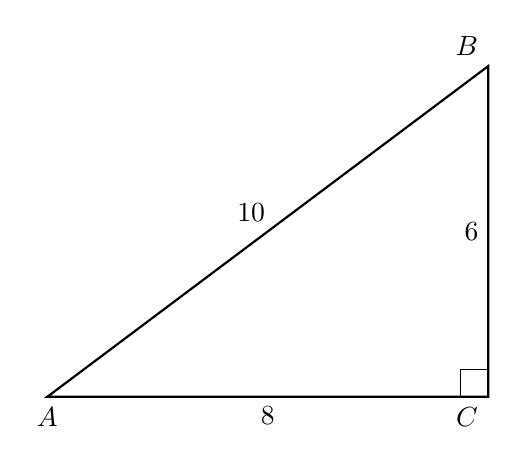
\begin{tikzpicture}[scale=0.7]
         \draw [thick]
         (0,0)node[below]{$A$}--
         (8,0)node[below left]{$C$}--
         (8,6)node[above left]{$B$}--cycle;
         \draw (8,0)++(-0.5,0)--++(0,0.5)--+(0.5,0);
         \node at (4,0)[below]{$8$};
         \node at (8,3)[left]{$6$};
         \node at (3.7,3)[above]{$10$};
       \end{tikzpicture}
     \end{multicols} \vspace{1cm}

   \item In a right triangle, the acute angles have the relationship $\sin (30)=\cos(x)$.\\[0.25cm]
     What is the value of $x$? \vspace{3cm}

   \item If $\sin (x-20)^\circ = \cos(60)^\circ$, what is the value of $x$? \vspace{5cm}

   \item Express each value to \emph{the nearest tenth}.  \vspace{0.5cm}
     \begin{multicols}{2}
       \begin{enumerate}
         \item $\sin 30^\circ = $ \vspace{1cm}
         \item $\cos 45^\circ =$
         \item $\tan^{-1} 1.732 = $ \vspace{1cm}
         \item $\cos^{-1} 0.866 =$
       \end{enumerate}
     \end{multicols}

 \newpage

   \item A flag pole is 60 feet away, and the angle of elevation to its top is $27^\circ$. To the \emph{nearest foot}, what is the height of the pole?\\
    \begin{tikzpicture}[scale=1.1]
      \draw [dashed] (10,0)--(0,0)--(10,4);
      \draw [thick, ->] (10,0)--(10,4);
      \draw (10,0)++(-0.3,0)--++(0,0.3)--+(0.3,0);
      \fill [lightgray] (0,0)--(0.75,0) arc [start angle=0, end angle=22, radius=0.75]--cycle;
      \node at (1,0)[below]{$27^\circ$};
      \node at (10,2)[right]{Flag Pole};
      \node at (5,0)[below]{60 feet};
    \end{tikzpicture} \vspace{4cm}

    \item Right $\triangle ABC$ is drawn with point $D$ on $\overline{AC}$. $m\angle BAC=50^\circ$, $m\angle BDC=75^\circ$, $m\angle C=90^\circ$, and $AC=20$. \\[0.5cm]
    ``Solve the triangle": Find $BC$, $BD$, $CD$, and $AD$. \vspace{0.5cm}
        \begin{flushright}
          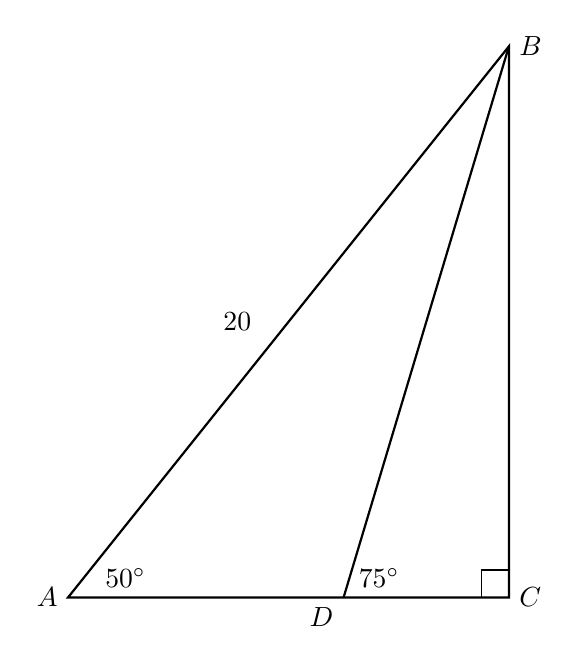
\begin{tikzpicture}[scale=0.7]
            \draw [thick] (-8,0)node[left]{$A$}
            --(0,0)node[right]{$C$}
            --(0,10)node[right]{$B$}--cycle;
            %\draw (0,0) circle [radius=5] node[below]{$O$};
            \draw [thick] (-3,0)node[below left]{$D$}--(0,10);
            \draw (0,0) ++(-180:0.5)-- ++(90:0.5)-- +(0:0.5);
            \node at (-4.5,5)[left]{$20$};
            \node at (-7.5,0)[above right]{$50^\circ$};
            \node at (-2.9,0)[above right]{$75^\circ$};
          \end{tikzpicture}
       \end{flushright}%\vspace{5cm}

\end{enumerate}
\end{document}
